\begin{figure}[htp!]
  \centering
  
\includegraphics[scale=0.22]{Esercizio14.1/Esercizio.jpg} 
\end{figure}
Considerando che la densità del platino è: $\rho_{\mathrm{Pt}}=21.4\,\mathrm{g}/\mathrm{cm}^3$ e $Z=78$. Come massa atomica prendo $A=156$ anche se ci sono numerosi isotopi stabili. Un calcolo più rigoroso includerebbe una media pesata. Richiamando la formula empirica di $I$ per grandi $Z$, si trova che $I\sim 10\,\mathrm{eV}\cdot Z=780\,\mathrm{eV}$.
\begin{figure}[htp!]
  \centering
  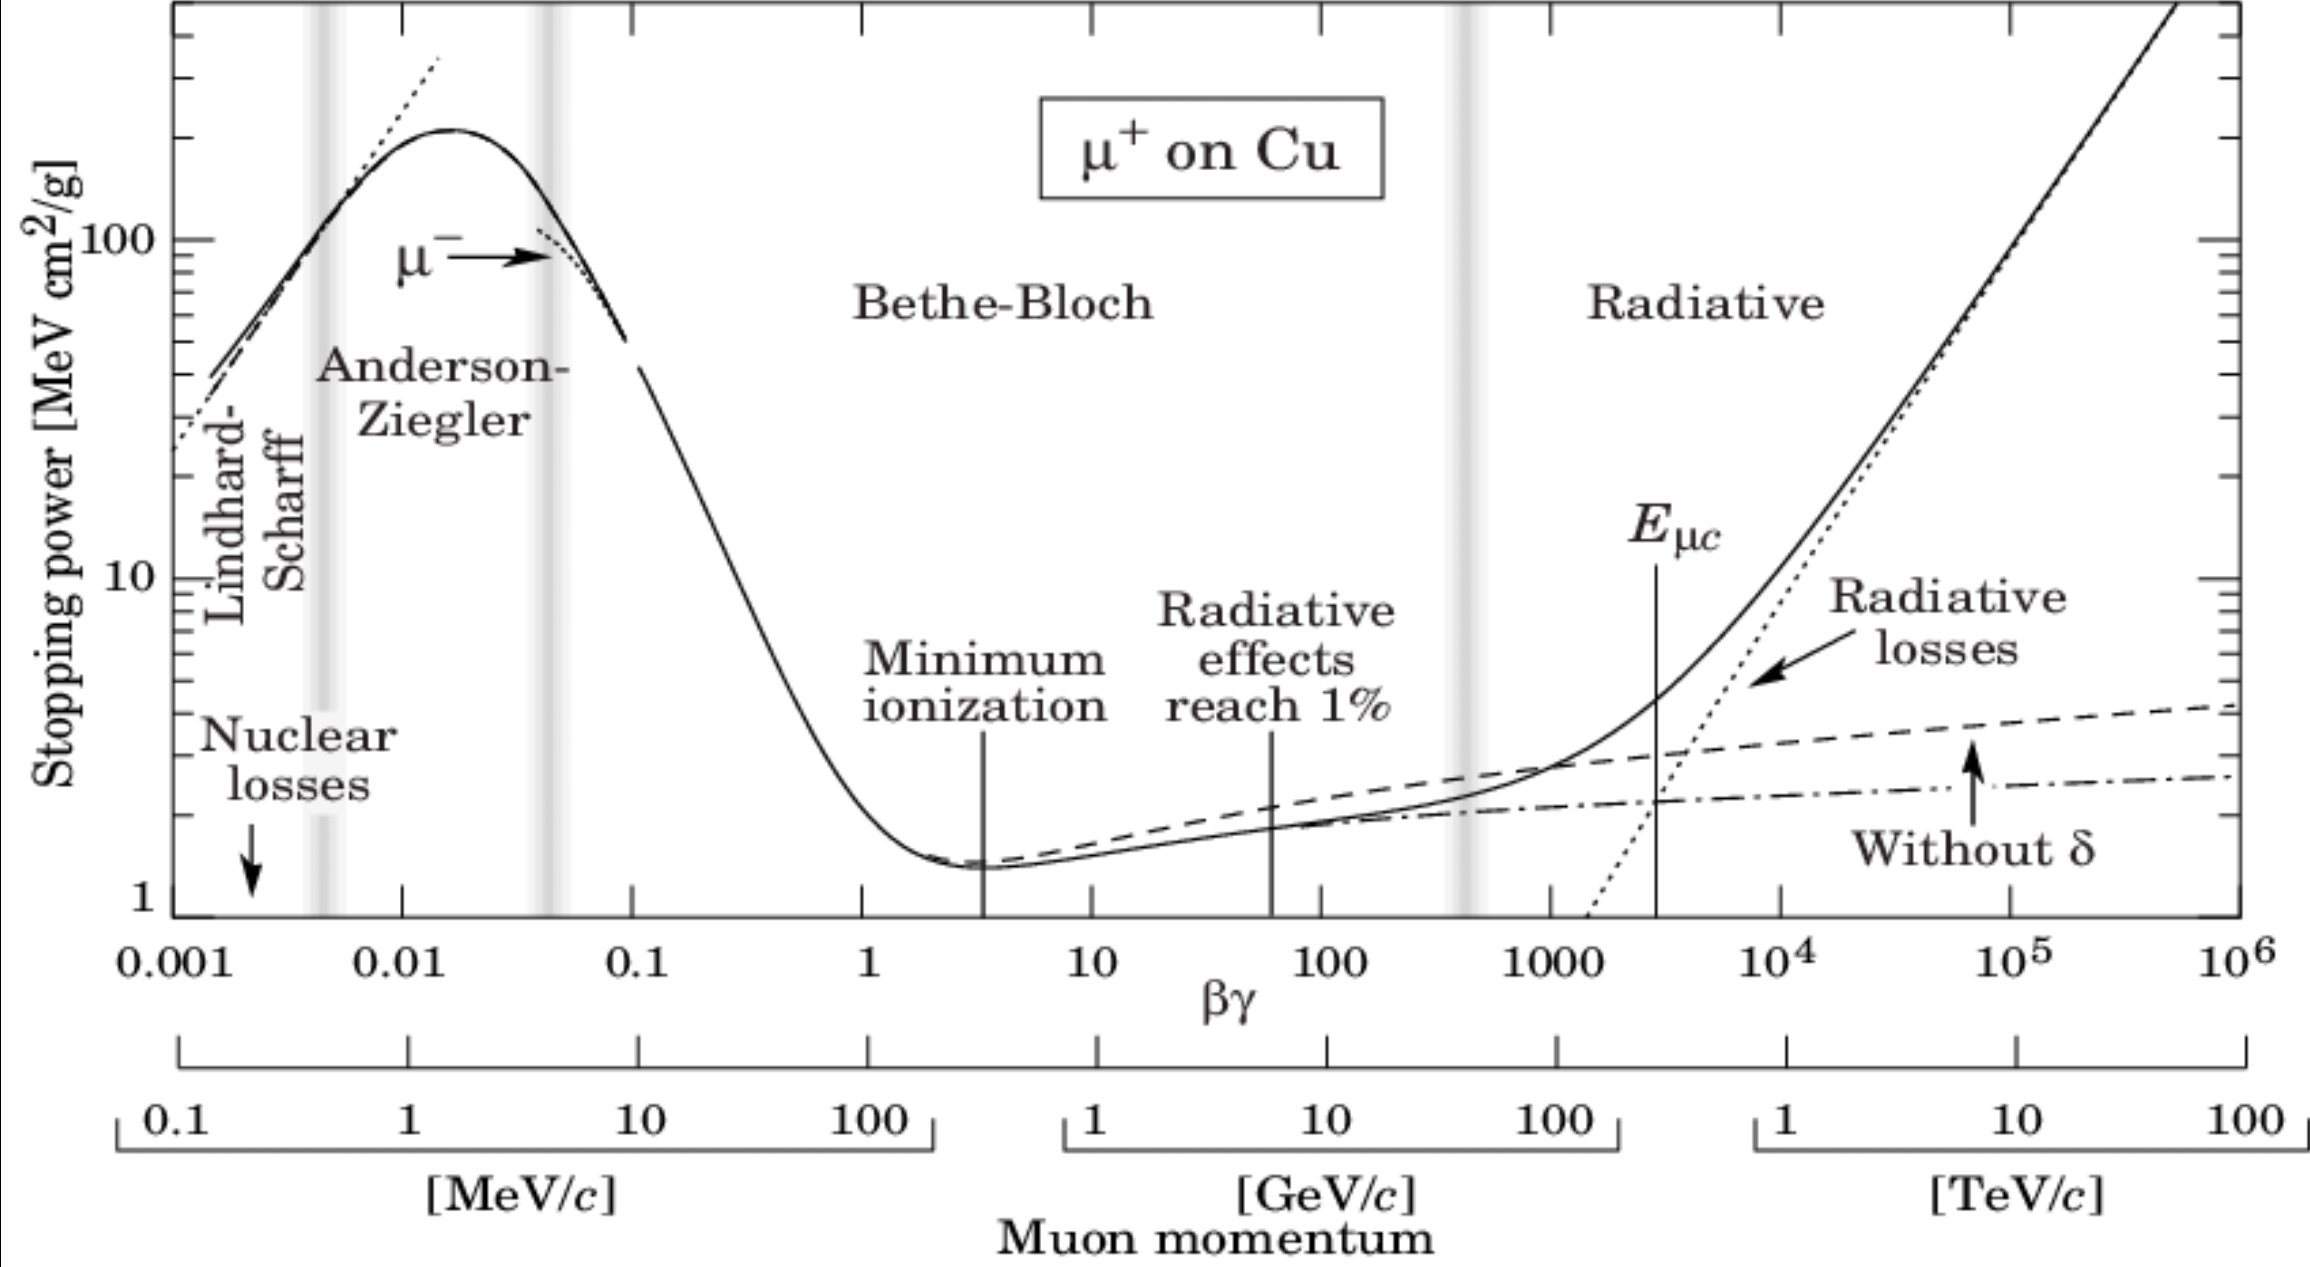
\includegraphics[scale=0.17]{Esercizio14.1/Bethe-Bloch.jpg} 
\end{figure}
Dopo aver calcolato il $\beta\gamma$ per le tre diverse particelle è possibile collocarle all'interno del grafico. Per l'elettrone:
\begin{equation}
    (\beta\gamma)_e=\frac{p}{m_e}\simeq1000
\end{equation}
Quindi siamo a regime ultrarelativistico e quindi possiamo trascurare il contributo della massa all'energi:
\begin{equation}
    E_e=\sqrt{m_e^2+p^2}\simeq p=500\,\mathrm{MeV}
\end{equation}
Per quanto riguarda il muone invece:
\begin{equation}
    (\beta\gamma)_\mu=\frac{p}{m_\mu}\simeq5 
\end{equation}
Sapendo che la massa del muone è: $m_\mu=105\,\mathrm{MeV}$. In questo caso quindi:
\begin{equation}
    E_\mu=\sqrt{m_\mu^2+p^2}=511\,\mathrm{MeV}
\end{equation}
Per il protone:
\begin{equation}
    (\beta\gamma)_p=\frac{p}{m_p}\simeq\frac{1}{2} 
\end{equation}
E quindi l'energia del protone:
\begin{equation}
    E_p\sqrt{m_p^2+p^2}=1063\,\mathrm{MeV}
\end{equation}
Partendo dal muone riconosciamo che si colloca molto vicino al minimo di ionizzazione quindi possiamo approssimare:
\begin{equation}
    \left(\frac{dE}{d(x\rho)}\right)_{\mu}\simeq1.5\,\frac{\mathrm{MeV}}{\mathrm{g}/\mathrm{cm}}
\end{equation}
Moltiplicando per la densità si trova:
\begin{equation}
    \left(\frac{dE}{dx}\right)_{\mu}=32.1\,\mathrm{MeV}/\mathrm{cm}
\end{equation}
Di conseguneza:
\begin{equation}
    \Delta E=-32.1\,\mathrm{MeV}\quad \Rightarrow\quad E_\mu'=479\,\mathrm{MeV} \quad \Rightarrow\quad p_\mu'=\sqrt{E_\mu'^2-m_\mu^2}=467\,\mathrm{MeV}
\end{equation}

Per il protone non si può fare la stessa approssimazione. Scrivendo la formula di Bethe-Bloch:
\begin{equation}
     \left(\frac{dE}{d(x\rho)}\right)_p=4 \pi r_e^2 m_e c^2 N_A\frac{Z}{A}\frac{z^2}{\beta^2}\left[\frac{1}{2} \ln \frac{2 \gamma^2 \beta^2 m_e c^2 T_{\max }}{\bar{I}^2}-\beta^2-\frac{\delta(\gamma \beta)}{2}\right] 
\end{equation}
Le correzioni dovute dalla $\delta$ sono piccole quindi possiamo trascurarlo. Ricordando che:
\begin{equation}
    T_\mathrm{max}=\frac{2\gamma^2\beta^2m_ec^2}{1+2\gamma m_e/M+(m_e/M)^2}\sim2\gamma^2\beta^2m_ec^2
\end{equation}
Con $M>>m_e$. Quindi si semplifica in:
\begin{equation}
    \left(\frac{dE}{d(x\rho)}\right)_p=4 \pi r_e^2 m_e c^2 N_A\frac{Z}{A}\frac{z^2}{\beta^2}\left[ \ln \frac{2\gamma^2\beta^2m_ec^2}{\bar{I}}-\beta^2\right]
\end{equation}
Sostituendo tutte le quantità e utilizzando l'approssimazione che mi chiude tutto il prefattore nel numero $0.15\,\frac{\mathrm{MeV}}{\mathrm{g}/\mathrm{cm}^2}$. Quindi:
\begin{equation}
    \left(\frac{dE}{dX}\right)_p=0.15\,\frac{\mathrm{MeV}}{\mathrm{g}/\mathrm{cm}^2}\frac{1}{\beta^2}\left[\ln \frac{2\gamma^2\beta^2m_ec^2}{\bar{I}}-\beta^2\right]=3.33\,\frac{\mathrm{MeV}}{\mathrm{g}/\mathrm{cm}^2}
\end{equation}
Quindi:
\begin{equation}
    \left(\frac{dE}{dx}\right)_p=71.2\,\frac{\mathrm{MeV}}{\mathrm{cm}}
\end{equation}
\begin{equation}
    \Delta E=-71.2\,\mathrm{MeV}\quad \Rightarrow\quad E_p'=992\,\mathrm{MeV} \quad \Rightarrow\quad p_p'=\sqrt{E_p'^2-m_p^2}=323\,\mathrm{MeV}
\end{equation}

Per quanto riguarda l'elettrone invece abbiamo già detto che è una particella a regime ultrarelativistico. La parte radiativa è quindi molto importante. Andando a guardare il sito consigliato dall'esercizio si vede che l'energia critica per il $Pt$ è di $7.59\,\mathrm{MeV}$ per gli elettroni. Significa che se l'energia nel nostro caso è molto maggiore di questa possiamo considerare solo il contributo radiativo, se invece è molto minore possiamo considerare solo il contributo collisionale. Nel caso in cui l'energia in gioco si a comparabile con questa energia critica bisogna considerare entrambi i contributi. Nel nostro caso abbiamo un elettrone di $E_e=500\,\mathrm{MeV}$ e quindi: $E_e>>E_{\text{crit}}$. Possiamo considerare solo termine radiativo. Quindi la perdita di energia è:
\begin{equation}
     \left(\frac{dE}{d(x\rho)}\right)_e=-\frac{E}{X_0}
\end{equation}
Dove:
\begin{equation}
    X_0=\frac{716.4 A}{Z(Z+1)\ln({287/\sqrt{z}})}\,\frac{\mathrm{g}}{\mathrm{cm}^2}=6.5\,\frac{\mathrm{g}}{\mathrm{cm}^2}
\end{equation}
E quindi:
\begin{equation}
    \left(\frac{dE}{dx}\right)_e=1666\,\frac{\mathrm{MeV}}{\mathrm{cm}}
\end{equation}
Verrebbe una $\Delta E=-1666\,\mathrm{MeV}$ che è impossibile. Siamo in una condizione in cui non vale $\frac{dE}{dx}x<<E$ e quindi non si può semplicemente moltiplicare lo spessore per la perdita di energia. Infatti bisogna tenere in considerazione che l'elettrone man mano che perde energia rallenta e quindi cambia anche il modo in cui perde energia. Quindi:
\begin{equation}
    \frac{dE}{E}=\frac{1}{X_0}dx\quad \Rightarrow\quad\int_{E_0}^{E'}\frac{dE}{E}=\frac{1}{X_0}\int_0^xdx
\end{equation}
Trovando come soluzione:
\begin{equation}
    E(x)=E_0e^{-\frac{x}{X_0}} \quad \Rightarrow\quad E(1\,\mathrm{cm})=25\,\mathrm{MeV}>>m_e \quad \Rightarrow\quad p_e'\simeq25\,\mathrm{MeV}
\end{equation}